\documentclass[14pt,aspectratio=1610]{beamer}
%\documentclass[12pt,aspectratio=1610,handout]{beamer}
\usepackage{csu-theme}
\usepackage{arrays}
\usepackage{linked-lists}
\usetikzlibrary{shapes.misc, backgrounds}

\tikzset{
  hashBucket/.style = {
    draw,
    rounded rectangle,
    align=center,
    anchor=west,
    font=\small,
    very thick,
    fill=CSUslate
  },
  chain bucket/.style = {
    draw,
    fill=CSUslate,
    very thick,
    rounded corners=2pt,
  },
  chain element/.style = {
    node of array,
    minimum height=8.5mm,
    fill=CSUcyan,
    text depth=.2ex
  }
}


\title{\Huge Hashing \& Hash Tables \\with Chaining}
\subtitle{CSCI 315: Data Structure Analysis\\Chapter 5 of \href{https://opendatastructures.org/ods-cpp.pdf}{Open Data Structures}}
%\author{Sean T. Hayes, Ph.D.}
\institute{Charleston Southern University}

%% Comment out date to use default (today)
% \date{March 25, 2025}
\subject{Software Programming}
%\keywords{}

\setlength{\parskip}{0.5em}

\graphicspath{{../imgs/}{../imgs/hashtables}}

\begin{document}

\begin{frame}
  \titlepage{}
\end{frame}

\section*{Intro}

\begin{frame}{Maps/Dictionary}
Map (dictionary) is a relation between a set of keys\\
and set of values.

\begin{figure}
\centering

\includegraphics[width=0.667\textwidth]{maping-keys-values}
\end{figure}
\end{frame}


\begin{frame}{Implementing Dynamic Maps/Dictionaries}

\begin{itemize}
\item
  We want a data structure in which finds/searches \\
  are very fast.
  \begin{itemize}
  \item
    As close to $O(1)$ as possible.
  \item
    With the minimum number of executed instructions per method.
  \end{itemize}
\item
  Insert and Deletes should be fast too.
\item
  Objects in a map have unique keys. A key may be:
  \begin{itemize}
  \item
    A single property/attribute value, or
  \item
    Created from multiple properties/values.
  \end{itemize}
\end{itemize}
\end{frame}

\begin{frame}{Implementing Dynamic Maps/Dictionaries}
We want to implement the map operations:\\
Insert, Delete, and Search/Find efficiently.

\begin{itemize}
\item
  \emph{Arrays}:
  \begin{itemize}
  \item
    accomplished in $O(1)$ time for integer keys of a known range.
  \item
    but are not space efficient (assumes we leave empty space for keys not currently in the map).
  \end{itemize}
\item
  \emph{Binary search trees}:
  \begin{itemize}
  \item
    can accomplish in $O(\log n)$ time
  \item
    are space efficient.
  \end{itemize}
\item
  \emph{Hash Tables}:
  \begin{itemize}
  \item
    A generalization of an array that under some reasonable assumptions is $O(1)$ for Insert/Delete/Search of a key.
  \end{itemize}
\end{itemize}
\end{frame}

\begin{frame}{Array Approach --- Example}
An application stores information about US citizens where \\the search key is their social security numbers (SSN).
\begin{itemize}
\item<2->
  You can use an array to hold references to all persons.
  \begin{itemize}
  \item
    Use an array with range 0 -- 999,999,999
  \item
    Using the SSN as a key, you have $O(1)$ access to any person.
  \end{itemize}
\item<3->
  Unfortunately, there are much fewer active keys (Social Security Numbers) than the array size (1 billion entries).
  \begin{itemize}
  \item
    Approximately \emph{450 million} SSNs have been issued since 1936.\\
    (net gain of 1 person every 22 seconds).
  \item
    For that many social security numbers, 55\% of the array would be unused.
  \end{itemize}
\end{itemize}
\end{frame}

\begin{frame}{Array Approach --- Example}
\begin{itemize}
\item
  Very useful data structure.
  \begin{itemize}
  \item
    Good for storing and retrieving key-value pairs.
  \item
    Not good for iterating through a list of items.
  \end{itemize}
\item
  Example application:\\
  Storing objects according to ID numbers.
  \begin{itemize}
    \item
      When the ID numbers are widely spread out.
    \item
      When you don't need to access items in ID order.
  \end{itemize}
\end{itemize}
\end{frame}

\begin{frame}{A Conceptual View of Hash Tables}
  \begin{figure}
  \centering
    \begin{tikzpicture}[node of array/.append style={minimum height=8mm,fill=CSUgold}]
      \ArrayLabel{Table}
      \ArrayNodeVertical{}
      \fill (val) circle(2pt);
      \node[block] (firstEl) [fit=(val)]{};

      \ArrayNodeVertical{}
      \fill (val) circle(2pt);
      \coordinate (ptr) at (val);
      \node[chain element, anchor=west, name=key] at ([xshift=2cm, yshift=8mm] prev.east) {key = 1};
      \node[chain element, anchor=west, name=valval] at ([xshift=-1pt] key.east) {val5};
      \begin{scope}[on background layer]
        \node[chain bucket, fit=(key) (valval)] (bucket) {};
        % \node[chain bucket] (bucket) [fit=(key) (valval)]{};
      \end{scope}
      \draw[link] (ptr) -- (bucket);
      \node[anchor=south] at(bucket.north) {Buckets};

      \ArrayNodeVertical{}
      \fill (val) circle(2pt);
      \coordinate (ptr) at (val);
      \node[chain element, anchor=west, name=key] at ([xshift=2cm] prev.east) {key = 2};
      \node[chain element, anchor=west, name=valval] at ([xshift=-1pt] key.east) {val4};
      \begin{scope}[on background layer]
        \node[chain bucket,fit=(key) (valval)] (bucket) {};
      \end{scope}
      \draw[link] (ptr) -- (bucket);


      \ArrayNodeVertical{}
      \fill (val) circle(2pt);

      \ArrayNodeVertical{}
      \fill (val) circle(2pt);
      \coordinate (ptr) at (val);
      \node[chain element, anchor=west, name=key] at ([xshift=2cm] prev.east) {key = 4};
      \node[chain element, anchor=west, name=valval] at ([xshift=-1pt] key.east) {val3};

      \node[chain element, anchor=west, name=key2] at ([xshift=5pt] valval.east) {key = 28};
      \node[chain element, anchor=west, name=valval2] at ([xshift=-1pt] key2.east) {val2};

      \begin{scope}[on background layer]
        \node[chain bucket,fit=(key) (valval) (key2) (valval2)] (bucket) {};
      \end{scope}
      \draw[link] (ptr) -- (bucket);

      \ArrayNodeVertical{}
      \fill (val) circle(2pt);

      \ArrayNodeVertical{}
      \fill (val) circle(2pt);

      \ArrayNodeVertical{}
      \fill (val) circle(2pt);
      \coordinate (ptr) at (val);
      \node[chain element, anchor=west, name=key] at ([xshift=2cm] prev.east) {key = 15};
      \node[chain element, anchor=west, name=valval] at ([xshift=-1pt] key.east) {val1};
      \begin{scope}[on background layer]
        \node[chain bucket,fit=(key) (valval)] (bucket) {};
      \end{scope}
      \draw[link] (ptr) -- (bucket);


      \draw [decorate, decoration = {brace,raise=5pt,amplitude=8pt}, very thick] ([xshift=-1cm]prev.south west) -- ([xshift=-1cm]firstEl.north west) node [pos=0.5,left=12pt,anchor=south, rotate=90] {hash value / index};

    \end{tikzpicture}
  \end{figure}
\end{frame}

% \begin{frame}{Hash Tables}
% \begin{itemize}
% \item
%   Hash Tables solve these problems by using a much smaller array and mapping keys with a hash function.
% \item
%   Let universe of keys $U$ and an array of size $m$. A hash function h is a function from $U$ to $0\ldots{}m$, that is:\\
%   $h : U \to 0\ldots{}m$
% \end{itemize}
% \begin{figure}
% \centering
% 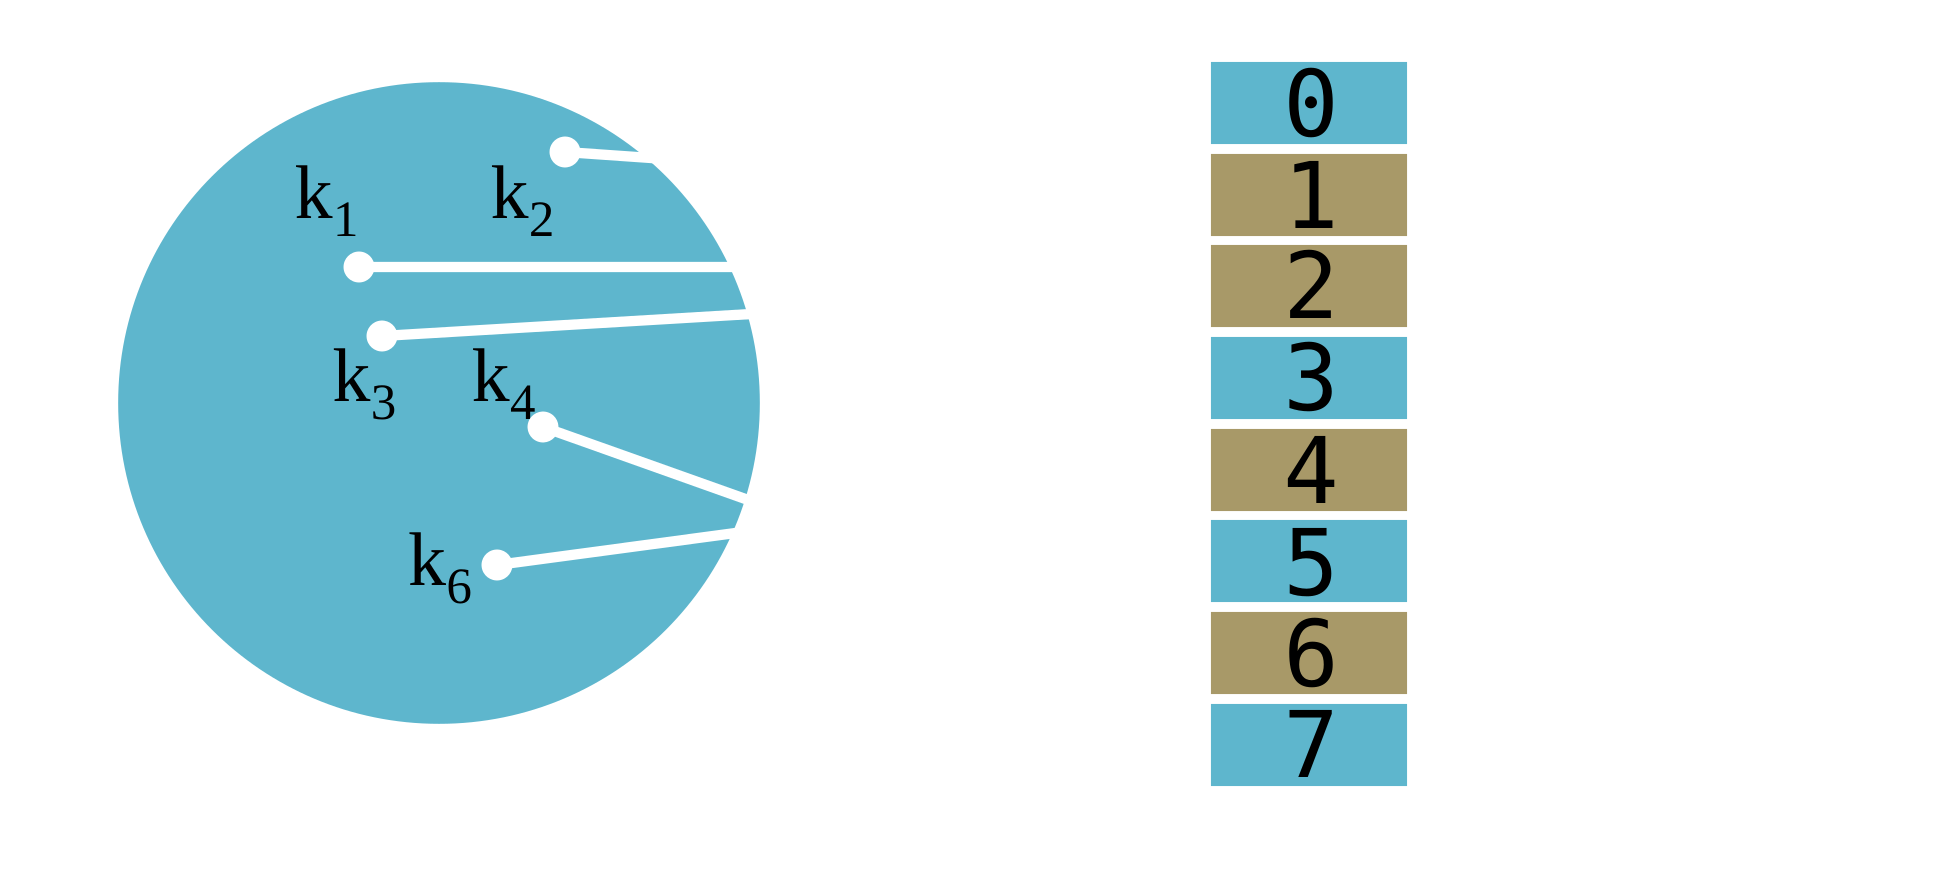
\includegraphics[width=0.7\textwidth]{keys-mapped-to-index}
% \end{figure}
% \end{frame}

\begin{frame}{Hash Tables}
  \begin{itemize}
  \item
    Hash Tables solve these problems by using a much smaller array and mapping keys with a hash function.
  \item
    Let universe of keys \(U\) and an array of size $m$. A hash function h is a function from $U$ to $0\ldots{}m$, that is:\\
    $h : U \to 0\ldots{}m$
  \end{itemize}
  \begin{figure}
    \centering
    \pgfdeclarelayer{background layer}
    \pgfdeclarelayer{foreground layer}
    \pgfsetlayers{background layer,main,foreground layer}
    
    \begin{tikzpicture}
      \newcommand\elName[1]{el####1}

      \foreach \n in {0,1,2,...,6}
      {
          \node[draw, minimum width=10mm, very thick, fill=CSUcyan, text=black, inner sep=0, minimum height=0.5cm] (el\n) at (0,3-\n*1/2) {\small\n};
      }

      \filldraw[color=white, fill=CSUcyan, very thick](-5,1.75) circle (1.5);
      \node[anchor=north] at (-5,1.75-1.5) {Universe of Keys (U)};

      % Seed the random number generator for reproducibility
      \pgfmathsetseed{57}

      

      % Loop to create 10 small circles
      \foreach \i in {1,...,8} {
        % Generate random angle and radius for polar coordinates within the large circle
        \pgfmathsetmacro{\angle}{random(0,360)}
        \pgfmathsetmacro{\radius}{sqrt(random()) * 1.25} % scale radius to stay within the larger circle

        % Convert polar to Cartesian coordinates
        \pgfmathsetmacro{\x}{\radius * cos(\angle) - 5}
        \pgfmathsetmacro{\y}{\radius * sin(\angle) + 1.75}
        \pgfmathsetmacro{\elNum}{int(mod(\i, 6))}
        

        % Draw the small circle and label it
        \fill[white] (\x,\y) circle (0.1cm); % Small circle with radius 0.3cm
        
        \draw[->, very thick] (\x, \y) to (el\elNum);
        
        \begin{pgfonlayer}{foreground layer}
          \node[text=black] at (\x-0.1,\y-0.1) {\small\(k_{\i}\)}; % Label the circle
        \end{pgfonlayer}

        %\node (el\elNum) {el{\elNum}};
      }

      % One extra circle at a specific spot.
      \pgfmathsetmacro{\x}{0.8 - 5}
      \pgfmathsetmacro{\y}{-0.9 + 1.75}
      \fill[white] (\x,\y) circle (0.1cm); % Small circle with radius 0.3cm
      \draw[->, very thick] (\x, \y) to (el6);
      \begin{pgfonlayer}{foreground layer}
        \node[text=black] at (\x-0.1,\y-0.1) {\small\(k_{10}\)}; % Label the circle
      \end{pgfonlayer}

      \node[anchor=west] at (el0.east) {\small \(h(k_6) = 0\)};
      \node[anchor=west] at (el1.east) {\small \(h(k_1) = h(k_7) = 1\)};
      \node[anchor=west] at (el2.east) {\small \(h(k_2) = h(k_8) = 2\)};
      \node[anchor=west] at (el3.east) {\small \(h(k_3) = h(k_9) = 3\)};
      \node[anchor=west] at (el4.east) {\small \(h(k_4) = 4\)};
      \node[anchor=west] at (el5.east) {\small \(h(k_5) = 5\)};
      \node[anchor=west] at (el6.east) {\small \(h(k_{10}) = 6\)};
    \end{tikzpicture}
  \end{figure}
\end{frame}

  
\section{Hashing}

\begin{frame}{Hash Index/Value}
\begin{itemize}
\item<+->
  A hash value or hash index is used to index the hash table (array).
\item<+->
  A hash function takes a key and returns a hash value/index.
  \begin{itemize}
  \item
    The hash index is an integer (to index an array).
  \end{itemize}
\item<+->
  The key is a value associated with a specific object being stored in the hash table.
  \begin{itemize}
  \item
    The key must remain constant for the lifetime of the object.
  \end{itemize}
\end{itemize}
\end{frame}

\begin{frame}{Generating Hash Codes}
\begin{itemize}
  \item<2->
    A key may not be an integer to directly used for \\hashing.\\
    For example,
    \begin{itemize}
      \item Floating-point numbers: (e.g., 3.14159, 23543.43, 3.997E-8)
      \item String values: (e.g., \texttt{"Alice"}, \texttt{"Dear diary"}, \texttt{":-)"})
      \item Objects of custom classes.
    \end{itemize}
  \item<3->
    In Java, every object has a \lstinline{hashCode()} method to return a hash code.
    \begin{itemize}
    \item
      A series of shifts, adds, and xors is performed on the key to produce pseudo-random numbers.
    \end{itemize}
  \item<4->
    Likewise, we need to make a hash-code function for each type we want to use as a key in our hash table.
\end{itemize}
\end{frame}

\begin{frame}[fragile]{Hash Functions \& \texttt{insert()}}
\begin{itemize}
\item
  Usage summary:\\
  \begin{lstlisting}[basicstyle=\ttfamily\small]
unsigned int hashCode (int key);
unsigned int hashCode (const std::string& key);
unsigned int hashCode (const ItemType& item);

template <typename Type>
unsigned int hash (const Type &key) {
  return hashCode(key) % TABLE_SIZE; // example
};
\end{lstlisting}
\item
  An insert method:
  \begin{lstlisting}[basicstyle=\ttfamily\small]
void insert (int key, itemType item) {
  const unsigned int HASH_VAL = hash(key);
  table[HASH_VAL] = item; // Incomplete
}
\end{lstlisting}
\end{itemize}
\end{frame}

\begin{frame}{The Mod (i.e., Modulo) Operator}
\begin{itemize}
\item
  The modulo is the remainder after integer division.
\item The modulo is the remainder.
  \setlength{\abovedisplayskip}{0pt}
  \begin{flalign}
    8 \bmod{5} & = 3\\
    9 \bmod{5} & = 4\\
    10 \bmod{5} & = 0\\
    15 \bmod{5} & = 0
  \end{flalign}
\item
  For keys $\bmod{} M$, multiples of $M$ give the same result, $0$.
  \begin{itemize}
  \item<+->
    But multiples of other numbers do not give the same result.
  \item<+->
    What if $M$ is a prime number such that the keys are rarely multiples of $M$?
  \end{itemize}
\end{itemize}
\end{frame}

\begin{frame}{Hash Tables: Insert Example}
For example, if we hash keys $0\ldots{}1000$ into a hash table\\
with $5$ entries and use $h (key) = key \bmod 5$, we get the following sequence of events.%
\vspace{-0.5em}
\center%
\begin{columns}[]%
  \column{0.3\textwidth}
  \center%
\begin{tikzpicture}[node of array/.append style = {minimum height=7mm}]
  \setcounter{arrayIndex}{0}
  \node[, name=prev] {key};

  % \onslide<-2>{
  %   \node[, left = 2cm of prev.west] {Insert $2$};
  % }
  % \onslide<3-4>{
  %   \node[, left = 2cm of prev.west] {Insert $21$};
  % }
  % \onslide<5-6>{
  %   \node[, left = 2cm of prev.west] {Insert $34$};
  % }
  % \onslide<7->{
  %   \node[, left = 2cm of prev.west] {Insert $54$};
  % }
  \node[, above = 0em of prev.north, anchor=south] {%
    \alt<-2>{Insert $2$}{%
      \alt<-4>{Insert $21$}{%
        \alt<-6>{Insert $34$}{%
          Insert $54$%
        }%
      }%
    }%
  };

  \foreach \key/\value [count=\i] in {
    % Key-Value Pairs
    {~/~},%
    {\only<4->{21}/\only<4->{\ldots{}}},%
    {\only<2->{2}/\only<2->{\ldots{}}},%
    {~/~},%
    {\only<6-7>{34}\only<8->{54}/\only<6-7>{\ldots{}}\only<8->{\color{red!70!black}\ldots{}}}%
  }{%
    \ifnum\i=5 % Last element: Allow it to change colors
      \alt<-7>{%
        \node[node of array, anchor=north, name=key] at ([yshift=1pt] prev.south) {\key};%
      }{%
        \node[node of array, anchor=north, name=key, fill=red] at ([yshift=1pt] prev.south) {\key};%
      }%
    \else % All but the last row
      \node[node of array, anchor=north, name=key] at ([yshift=1pt] prev.south) {\key};%
    \fi%
    \node[node of array, right = of key.east, xshift=-1pt, name=valData, minimum width=1.5cm] {\value};%
    \ifnum\i=1 % First element
      \node[, above = 2pt of valData] {value};%
    \fi%
    \node[array index, anchor=east] at ([xshift=-1pt] key.west) {[\thearrayIndex]};%
    \node[block] (prev) [fit=(key)]{};%
    \stepcounter{arrayIndex}%
  }
\end{tikzpicture}
%
% \begin{columns}[T]%
%   \column{0.2\textwidth}\center%
%     Insert $2$\\[0.5em]
%     \small%
%     \begin{tabular}{c|c|c|}
%       \multicolumn{1}{c}{} & \multicolumn{1}{c}{key} & \multicolumn{1}{c}{data}\\
%     \cline{2-3}
%       \texttt{0} &   & \\
%     \cline{2-3}
%       \texttt{1} &   & \\
%     \cline{2-3}
%       \texttt{2} & \onslide<2->{$2$} & \onslide<2->{$\cdots$}\\
%     \cline{2-3}
%       \texttt{3} &   & \\
%     \cline{2-3}
%       \texttt{4} &   & \\
%     \cline{2-3}
%     \end{tabular}

%   \onslide<3->{%
%     \column{0.2\textwidth}\center%
%       Insert $21$\\[0.5em]
%       \small%
%       \begin{tabular}{c|c|c|}
%         \multicolumn{1}{c}{} & \multicolumn{1}{c}{key} & \multicolumn{1}{c}{data}\\
%       \cline{2-3}
%         \texttt{0} &   & \\
%       \cline{2-3}
%         \texttt{1} & \onslide<4->{$21$} & \onslide<4->{$\cdots$} \\
%       \cline{2-3}
%         \texttt{2} & $2$ & $\cdots$\\
%       \cline{2-3}
%         \texttt{3} &   & \\
%       \cline{2-3}
%         \texttt{4} &   & \\
%       \cline{2-3}
%       \end{tabular}}

%   \column{0.2\textwidth}\center%
%     \onslide<5->{%
%       Insert $34$\\[0.5em]
%       \small%
%       \begin{tabular}{c|c|c|}
%         \multicolumn{1}{c}{} & \multicolumn{1}{c}{key} & \multicolumn{1}{c}{data}\\
%       \cline{2-3}
%         \texttt{0} &   & \\
%       \cline{2-3}
%         \texttt{1} & $21$ & $\cdots$ \\
%       \cline{2-3}
%         \texttt{2} & $2$ & $\cdots$\\
%       \cline{2-3}
%         \texttt{3} &   & \\
%       \cline{2-3}
%         \texttt{4} & \onslide<6->{$34$} & \onslide<6->{$\cdots$}\\
%       \cline{2-3}
%       \end{tabular}}

%   \column{0.2\textwidth}\center
%     \onslide<7->{%
%       Insert $54$\\[0.5em]
%       \small%
%       \begin{tabular}{c|c|c|}
%         \multicolumn{1}{c}{} & \multicolumn{1}{c}{key} & \multicolumn{1}{c}{data}\\
%       \cline{2-3}
%         \texttt{0} &   & \\
%       \cline{2-3}
%         \texttt{1} & $21$ & $\cdots$ \\
%       \cline{2-3}
%         \texttt{2} & $2$ & $\cdots$\\
%       \cline{2-3}
%         \texttt{3} &   & \\
%       \cline{2-3}
%         \texttt{4} & \alt<-7>{$34$}{\color{red!50}\xout{$34$}} \onslide<8->{$54$} & $\cdots$\\
%       \cline{2-3}
%       \end{tabular}}
% \end{columns}
\column{0.5\textwidth}
  \center%
  \onslide<9->{%
    There is a \emph{collision} in the array at index \texttt{4}.\\
    How can we solve this issue?}
\end{columns}
\end{frame}

\begin{frame}{Reducing Collisions}
Ideally, \lstinline{hash(key)} has two properties:
\begin{enumerate}
  \item<2->
    Consistent: if \lstinline{x == y}, then \lstinline{hash(x) == hash(y)}
  \item<3->
    No Collisions: if \lstinline{x != y}, then \lstinline{hash(x) != hash(y)}
\end{enumerate}

\onslide<4->{
If the table size is less than the range of possible keys, property 2 cannot be met for all keys.
}

\onslide<5->{
Therefore, we have two goals:
\begin{enumerate}
  \item<6->
    Make collisions as unlikely as possible by choosing a good hashing function.
  \item<7->
    Effectively handle collisions when they occur.
\end{enumerate}}
\end{frame}

\begin{frame}{Choosing a Hash Function}
\begin{itemize}[<+->]
  \item
    Many programming languages (including Java) have built-in hash functions.
  \item
    The performance of the hash table depends on having a hash function that evenly distributes the keys.\\
    Uniform hashing is the ideal target.
  \item
    Choosing a good hash function requires accounting for the kind of data that will be used.
  \item
    One must account for the statistical distribution of keys.
    \begin{itemize}
    \item
      For example, choosing the first letter of a last name will likely cause lots of collisions depending on the nationality of the population.
    \end{itemize}
\end{itemize}
\end{frame}

\begin{frame}{Choosing a Hash Function}
  \begin{figure}
    \centering
    \caption{Distribution of the people's surname initial letter according to the 2010 US Census.}
    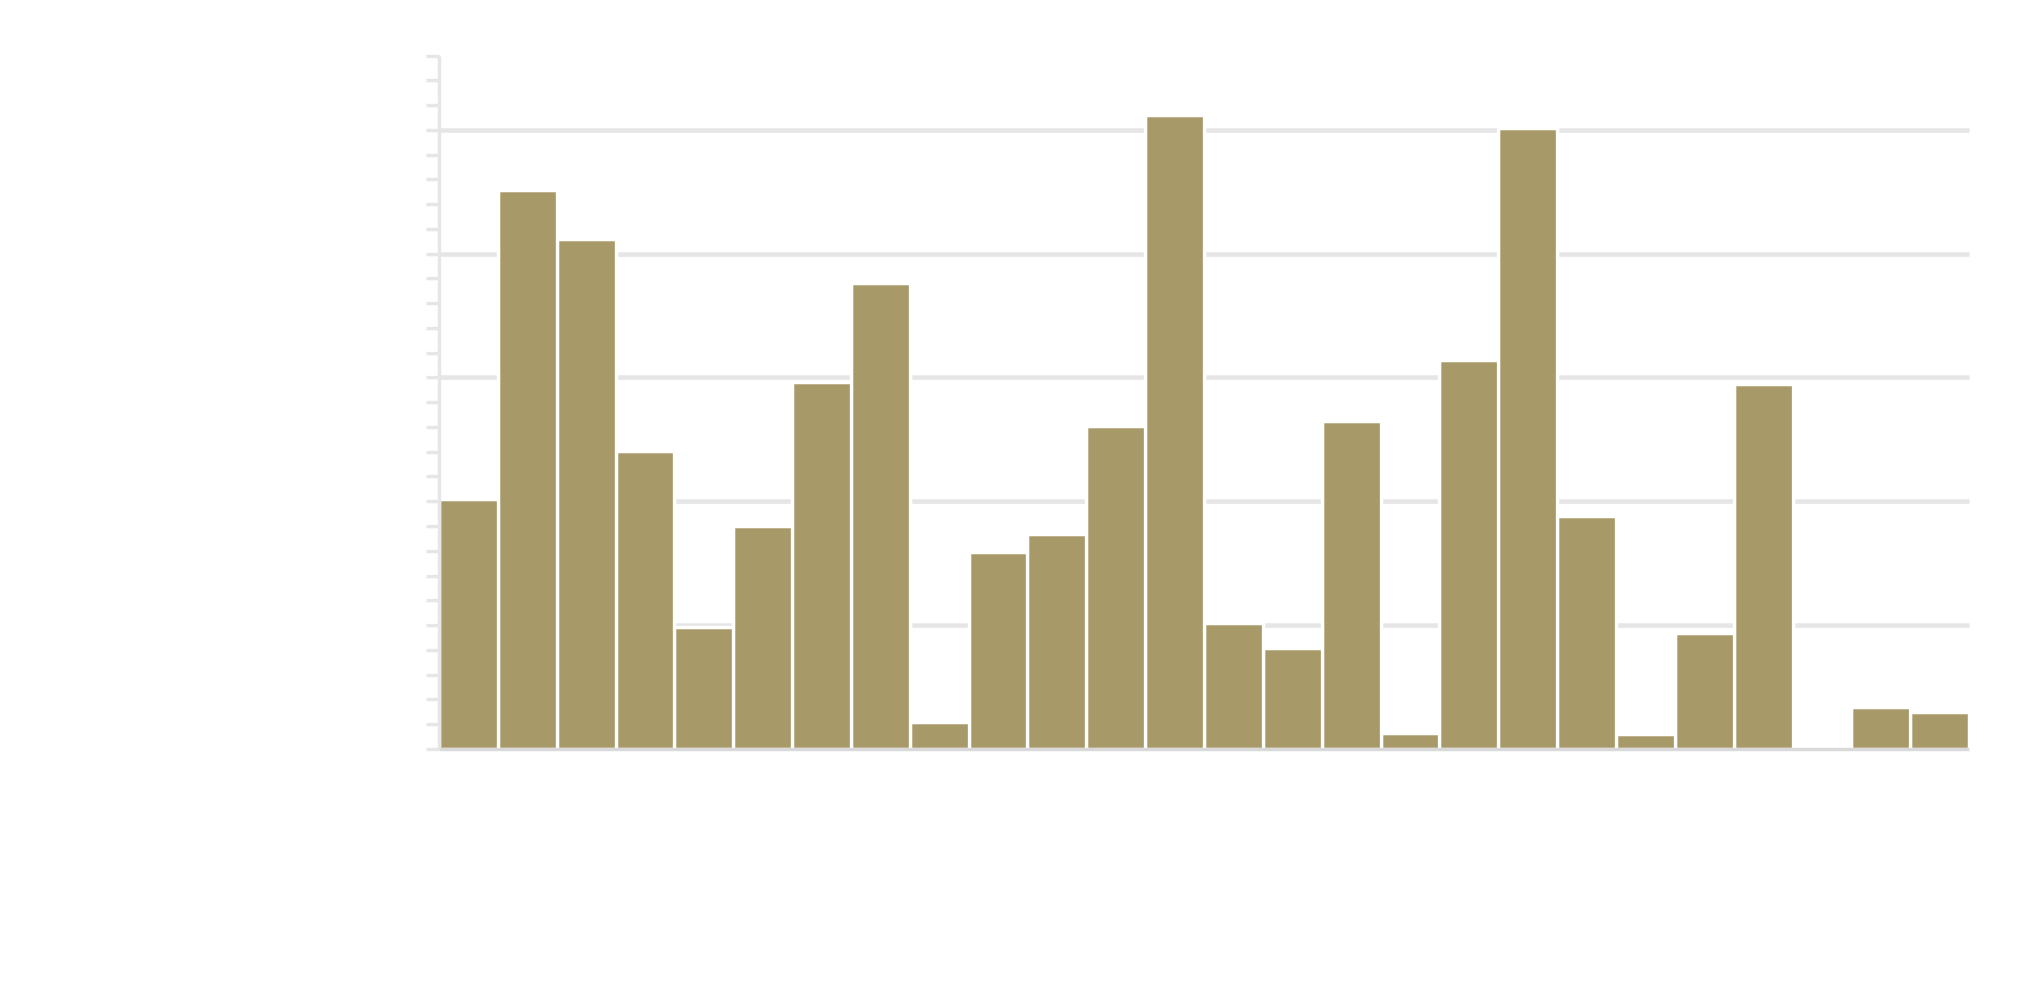
\includegraphics[width=0.9\textwidth]{FirstLetterOfLastNames}
  \end{figure}
\end{frame}

\begin{frame}{Choosing a Hash Function}
Some hashing methods that convert a hash code, $f(v)$, \\into an array index:
\begin{itemize}
  \item<2->
    Division/Modulo Method:
    \begin{itemize}
    \item
      Given: $m$ is the array size, which usually should be \emph{prime number}.\\
    \item
      $h(v) = f(v) \bmod{}m$
    \end{itemize}
  \item<3->
    Multiplicative Method:
    \begin{itemize}
    \item
      Given, $m$ is the array size (usually a power of 2).\\
      $p$ is a randomly chosen \emph{prime}, greater than $m$ (often $2^{31} - 1$) \\
      $a$ and $b$ are random positive integers that are less than $m$.\\
    \item
      $h(v) = \left(\left(a \cdot f(v) + b\right) \bmod{} p\right) \bmod{} m$
    \end{itemize}
\end{itemize}
\end{frame}


\begin{frame}{Prime Number Distribution}
\begin{columns}[T]
\column{0.7\textwidth}
For example, assume:
\begin{itemize}
  \item
    Key values, $v$, are multiples of $5$ from $5$ to $245$.\\
    (5$, 10, 15, 20, 25, \ldots, 245$).
  \item
    The array size (and divisor), $m$, is $7$.
  \item
    Then, the hash values will be evenly distributed from $0$ to $6$ for the keys.
  \item
    If $m$ was $5$, then you would have what kind of distribution?
\end{itemize}
\column{0.3\textwidth}%
\begin{table}\centering\small%
  \begin{tabular}{c c}%
  \hline%
    $v \bmod{} m$ & Total\\
  \hline
    0  &  7\\
    1  &  7\\
    2  &  7\\
    3  &  7\\
    4  &  7\\
    5  &  7\\
    6  &  7\\
    (blank)  &  \\
  \hline
    Grand Total & 49\\
  \hline
  \end{tabular}
\end{table}
\end{columns}
\end{frame}


\begin{frame}{Choosing Hash Function}
\begin{itemize}
  \item
    If the keys are non-random (e.g., part numbers), \\
    do the following for better distributions:
    \begin{itemize}
    \item
      Use all unique data to contribute to the hash function.
    \item
      Consider folding --- sum the natural (or arbitrary) groups of digits in the key.
    \item
      Exclude redundant or non-data (e.g., checksum values).
    \item
      Exclude information that may change!
    \end{itemize}
  \item
    Analyze your expected key values (or some representative subset) to ensure your hash function gives a good distribution!
\end{itemize}
\end{frame}

\begin{frame}{Dealing with Collisions}
A problem arises when we have two keys that hash in the same array entry --- this is called a \emph{collision}.

\onslide<2->{There are two ways to resolve collision:}
\begin{itemize}
  \item<3->
    \emph{Hashing with Chaining} (a.k.a., ``Separate Chaining''):\\
    Every hash-table entry contains a pointer to a linked list of keys that hash in the same entry.
  \item<4->
    \emph{Hashing with Open Addressing}:\\
    Every hash-table entry contains only one key. If a new key hashes to a filled table entry, systematically examine other table entries until an empty entry is found for the new key.
\end{itemize}
\end{frame}

\section{Chaining}
\begin{frame}{Hashing with Chaining}
  \alt<1>{
    \textbf{Problem}: Collisions\\
    (e.g., the keys $34$ and $54$ both hash to \texttt{4}).
  }{
    \textbf{Solution}: Place keys that hash in the same hash-table \\
    entry in the same \emph{chain} (linked list) or \emph{bucket} (array).
  }
  \vspace{-0.75em}
% \begin{columns}[T]%
% \column{0.4\textwidth}
\onslide<3->
\begin{figure}
\centering
\caption{\onslide<4->{\normalsize Insert \alt<-6>{$54$}{$101$}}\vspace{-0.25em}}\vspace{-0.25em}

\begin{tikzpicture}[node of array/.append style={minimum height=8.6mm,fill=CSUgold},
    link pointer of list/.append style={minimum height=6mm, minimum width=4mm,},
    node of list/.append style={minimum height=6mm, minimum width=9mm, inner sep=1pt},
    additional node of list/.append style={fill=CSUslate, minimum width=7mm}
  ]
  \ArrayLabel{}%\small{Table}
  
  \ArrayNodeVertical{}
  \fill (val) circle(2pt);
  \coordinate (ptr) at (val);

  \ArrayNodeVertical{}
  \fill (val) circle(2pt);
  \coordinate (ptr) at (val);
  \LinkedNode{1, ~}

  \node[, name=keyText, anchor=north, inner sep=0pt] at ([yshift=10mm]firstElValue.north) {key};
  \node[, name=valueText, anchor=north west, inner sep=0pt] at ([xshift=6pt]keyText.north east) {value};
  \draw[link] (keyText) to (firstElValue);
  \draw[link] (valueText) to (lastElValue);

  \onslide<8->{
    \LinkedNode{101, ~}
  }

  \ArrayNodeVertical{}
  \fill (val) circle(2pt);
  \coordinate (ptr) at (val);
  \LinkedNode{2, ~}

  \ArrayNodeVertical{}
  \fill (val) circle(2pt);
  \coordinate (ptr) at (val);

  \ArrayNodeVertical{}
  \fill (val) circle(2pt);
  \coordinate (ptr) at (val);

  \LinkedNode{34, ~}%
  \node[block] (el34) [fit=(last)]{};
  \onslide<5->{
    \LinkedNode{54, ~}%
    \onslide<6->
    {
      \draw [decorate, decoration = {brace,raise=2pt,amplitude=7pt}, very thick] (el34.north west) -- (last.north east) node [pos=0.5,above=8pt,anchor=south] {chain};
    }
  }

\end{tikzpicture}
% \onslide<3>{}

% % \includegraphics[width=0.9\textwidth]{chain-example-insert1}
% \end{figure}

% \column{0.4\textwidth}
% % \pause{}
% \begin{figure}
% \centering
% \caption{Insert $101$}\vspace{1.5em}
% \includegraphics[width=0.9\textwidth]{chain-example-insert2}
\end{figure}
% \end{columns}
\end{frame}

\begin{frame}{Hashing with Chaining}

\begin{figure}
\centering
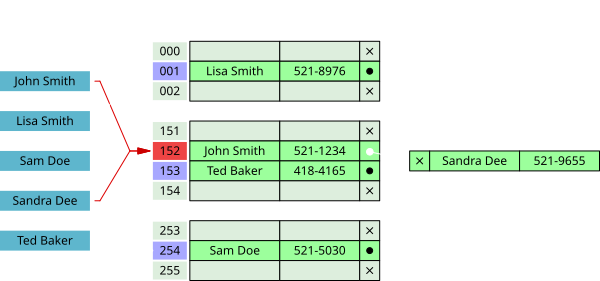
\includegraphics[width=0.95\textwidth]{chain-example-string-wikimedia}
\caption{\footnotesize By Jorge Stolfi -- Own work, CC BY-SA 3.0, \href{https://commons.wikimedia.org/w/index.php?curid=6472274}{https://commons.wikimedia.org/w/index.php?curid=6472274}}
\end{figure}
\end{frame}

\section{Performance}

\begin{frame}{Performance of Hashing with Chaining}
\begin{block}{Running-time performance for hash tables with chaining}
\begin{itemize}
  \item
    Insert: It takes $O(1)$ time to compute the hash function and insert at the head of the linked list.
  \item
    Search: It is proportional to max length of the linked lists.
  \item
    Delete: Same as search.
\end{itemize}
\end{block}

\pause{}
Therefore, in the unfortunate event that we have a ``bad'' hash function all $n$ keys may hash in the same table entry giving an $O(n)$ run-time!

\pause{}
So, we must create a ``good'' hash function.
\end{frame}

\section*{Lab 18}
\begin{frame}{Lab 18: Hash Tables with Chaining}
\begin{center}\Large
Let's take a look at the lab based on today's lecture.
\end{center}
\end{frame}

\end{document}